\documentclass{standalone}

\usepackage{tikz,pgf}

\begin{document}


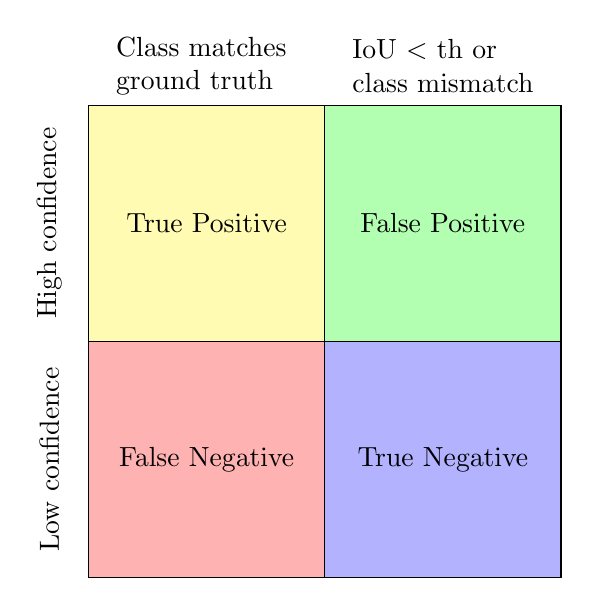
\begin{tikzpicture}
    \draw[draw=black,fill=yellow!30] (0,0) rectangle (3,3);
    \draw[draw=black,fill=green!30] (3,0) rectangle (6,3);
    \draw[draw=black,fill=red!30] (0,-3) rectangle (3,0);
    \draw[draw=black,fill=blue!30] (3,-3) rectangle (6,0);
    
    \node at (1.5,1.5) {True Positive};
    \node at (4.5,1.5) {False Positive};
    \node at (1.5,-1.5) {False Negative};
    \node at (4.5,-1.5) {True Negative};

    \node[text width=2.5cm] at (1.6,3.5) {Class matches ground truth};
    \node[text width=2.5cm] at (4.6,3.5) {IoU \begin{math}<\end{math} th or class mismatch};
    \node[rotate=90] at (-0.5,1.5) {High confidence};
    \node[rotate=90] at (-0.5,-1.5) {Low confidence};
\end{tikzpicture}


\end{document}